\section{Die Landkreise und Regierungsbezirke sortiert nach dem Gemeindeschlüssel}
In \autoref{fig:distribution_AdmUnitId} sind die Landkreise und Regierungsbezirke entsprechend der lexikographischen Ordnung der Gemeindeschlüssel eingefärbt. Anhand der Farbe der Landkreise/Regierungsbezirke lässt sich die grobe Nord-Süd und Ost-West Sortierung erkennen, die eine Sortierung der Liste der Landkreise/Regierungsbezirke nach Gemeindeschlüsseln ergibt.
\begin{figure}[H]
    \centering
    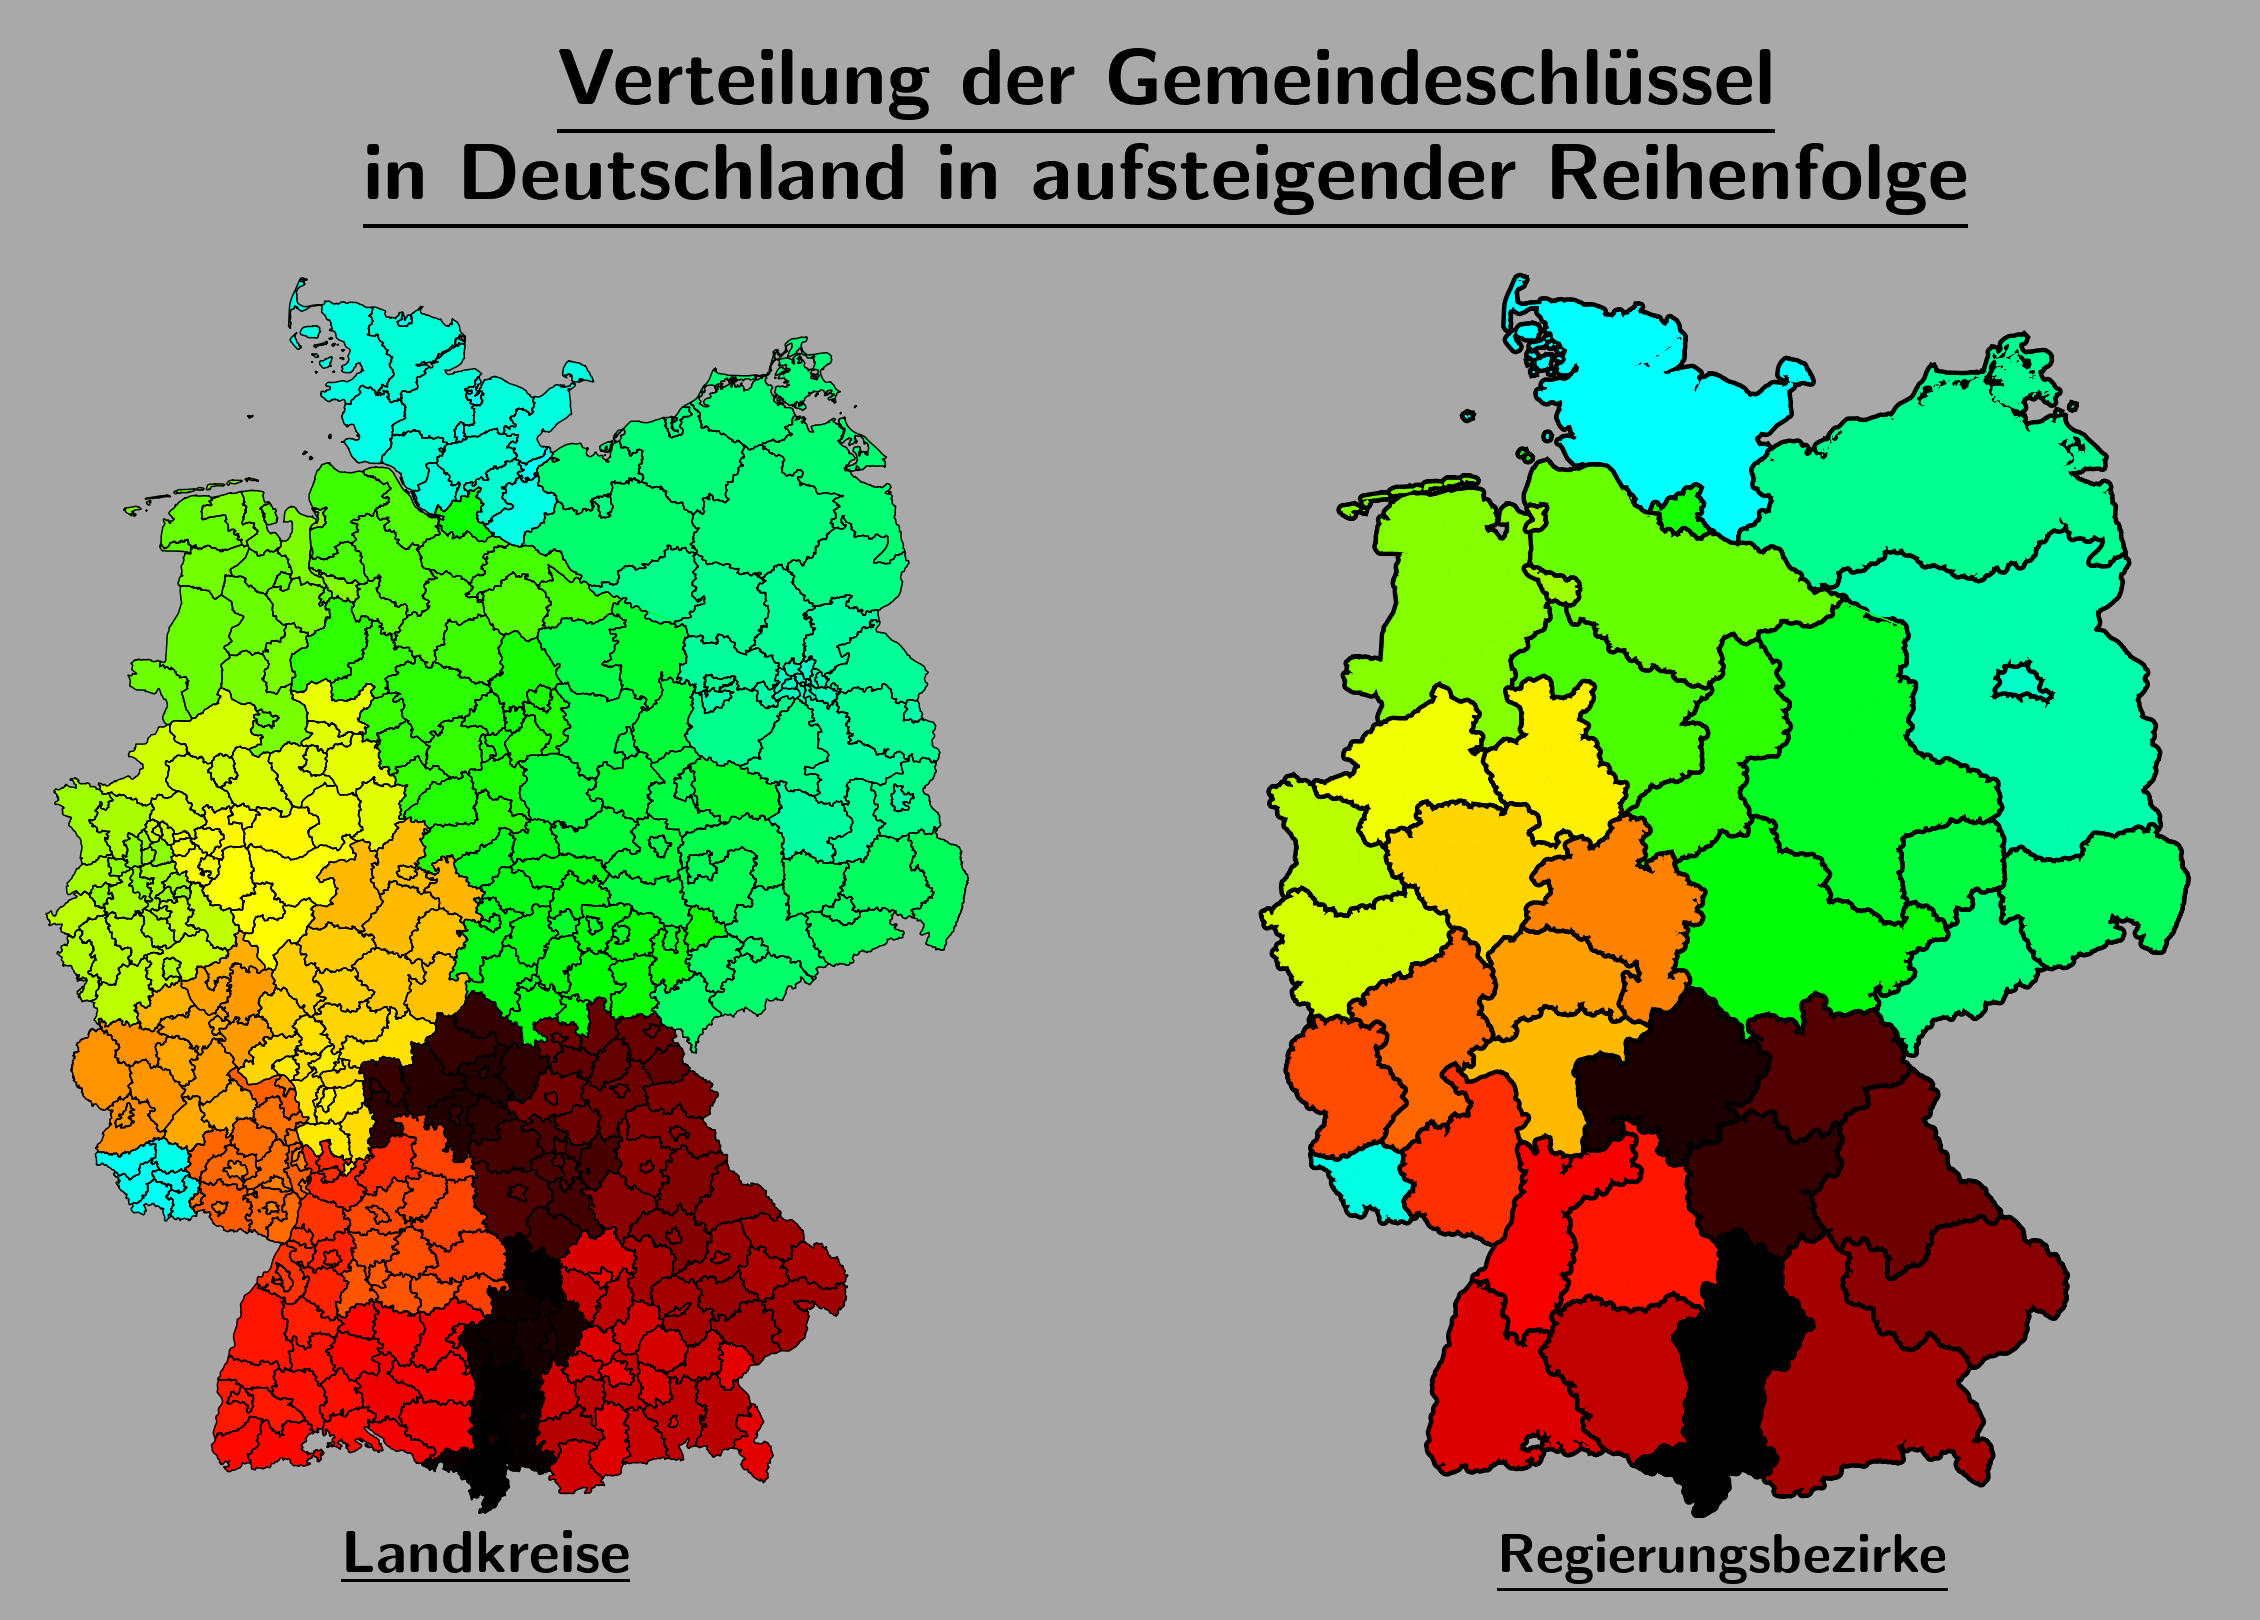
\includegraphics[width = 0.95\textwidth]{figures/Ergebnisse/districts_and_counties_by_AdmUnitID.png}
    \caption{Die Landkreise und Regierungsbezirke eingefärbt nach der lexikographischen Größe ihres Gemeindeschlüssels.}
    \label{fig:distribution_AdmUnitId}
\end{figure}